%!TEX root = main.tex

\section{Background} % (fold)
\label{sec:background}

The original Spark model is a centralized system.
Client send job to the driver, and driver will split into tasks and send to multiple workers.
When worker finishes the task, it will send it back to driver.
If any worker is failed, the driver will notice it and react to the failure, such at recompute on other workers.
Driver is efficient on computation, but also introduces a disadvantage to the cluster, single point failure.
It's hard and slow to recover the driver node, and the system becomes unavailable during this time.

\begin{figure}[htb]
    \centering
    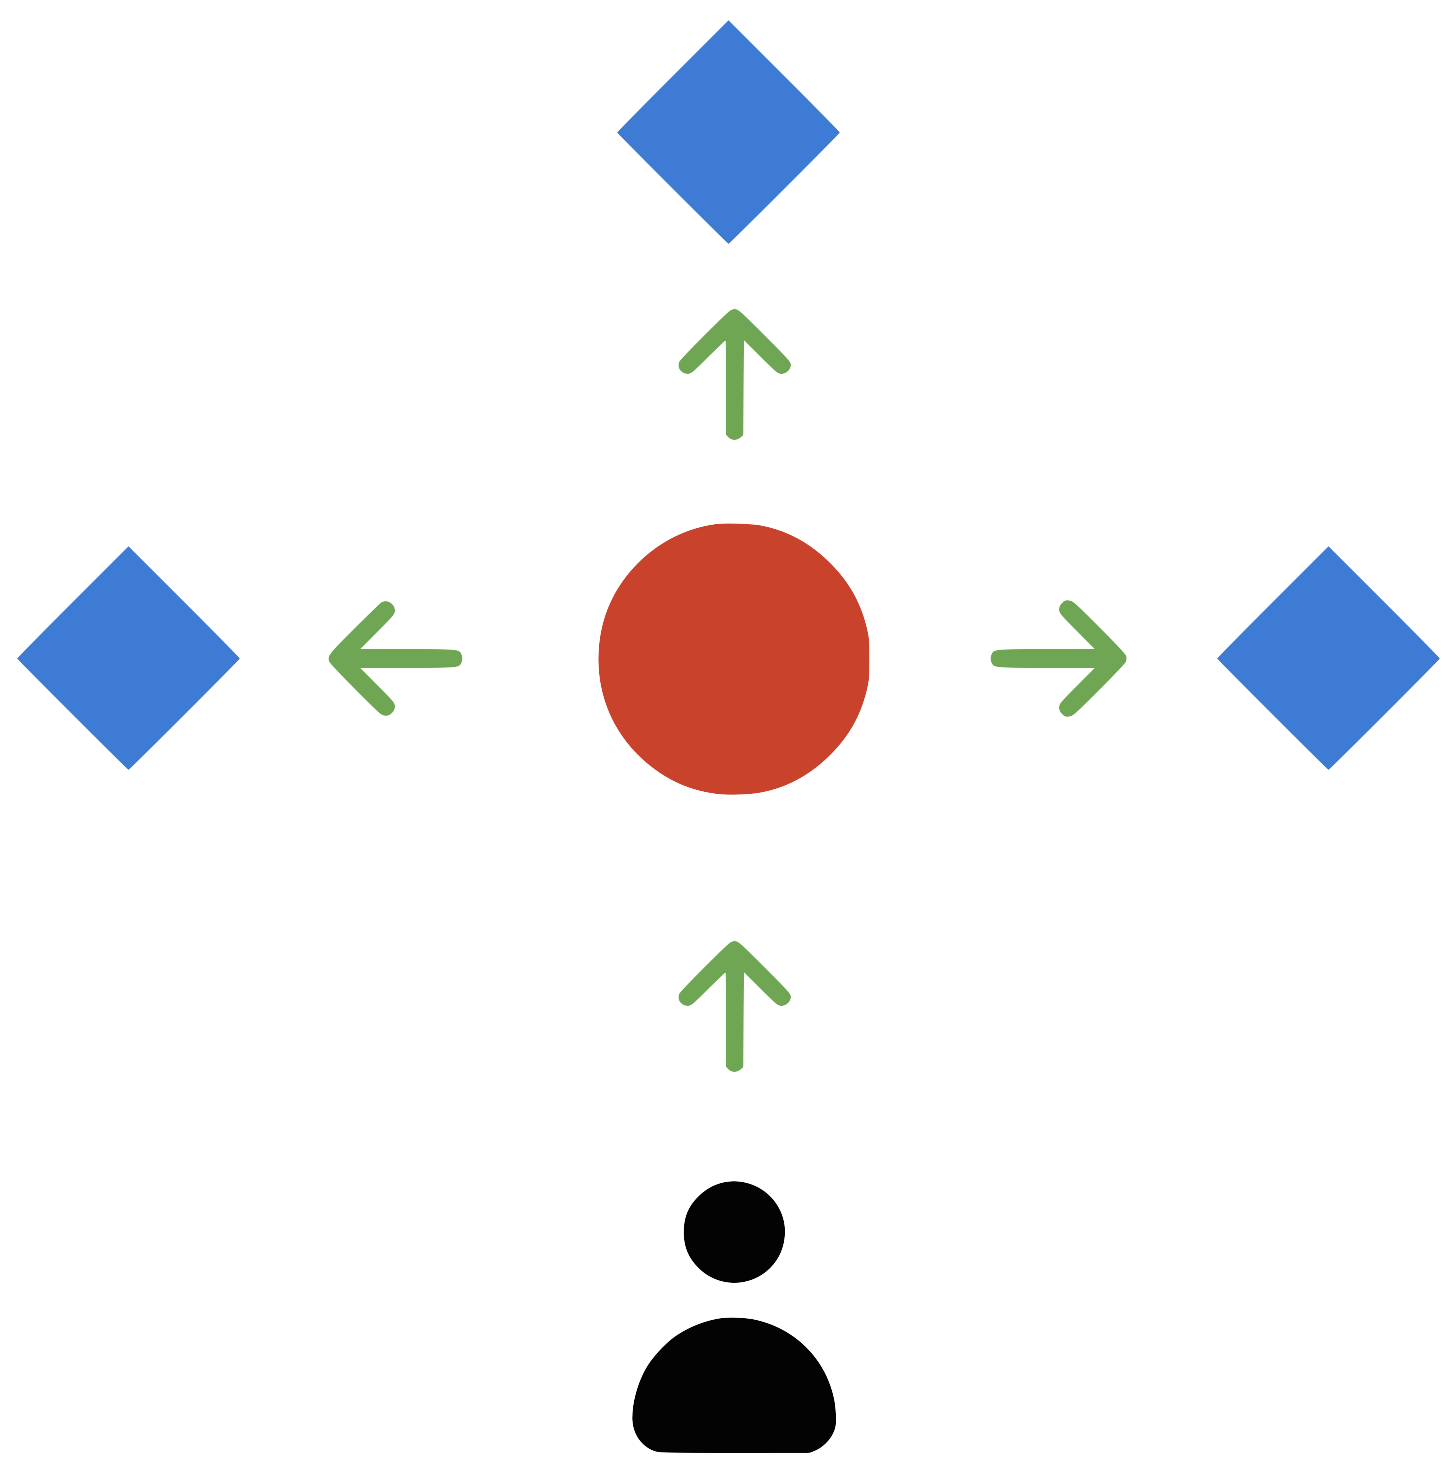
\includegraphics[width=0.5\textwidth]{images/original_model.png}
    \caption{Original Spark Model}\label{fig:original_model}
\end{figure}

The basic idea of Spark Driverless is by removing the Driver entirely and communicate by sending message,
we can achieve single-point-failure-free.

\begin{figure}[htb]
    \centering
    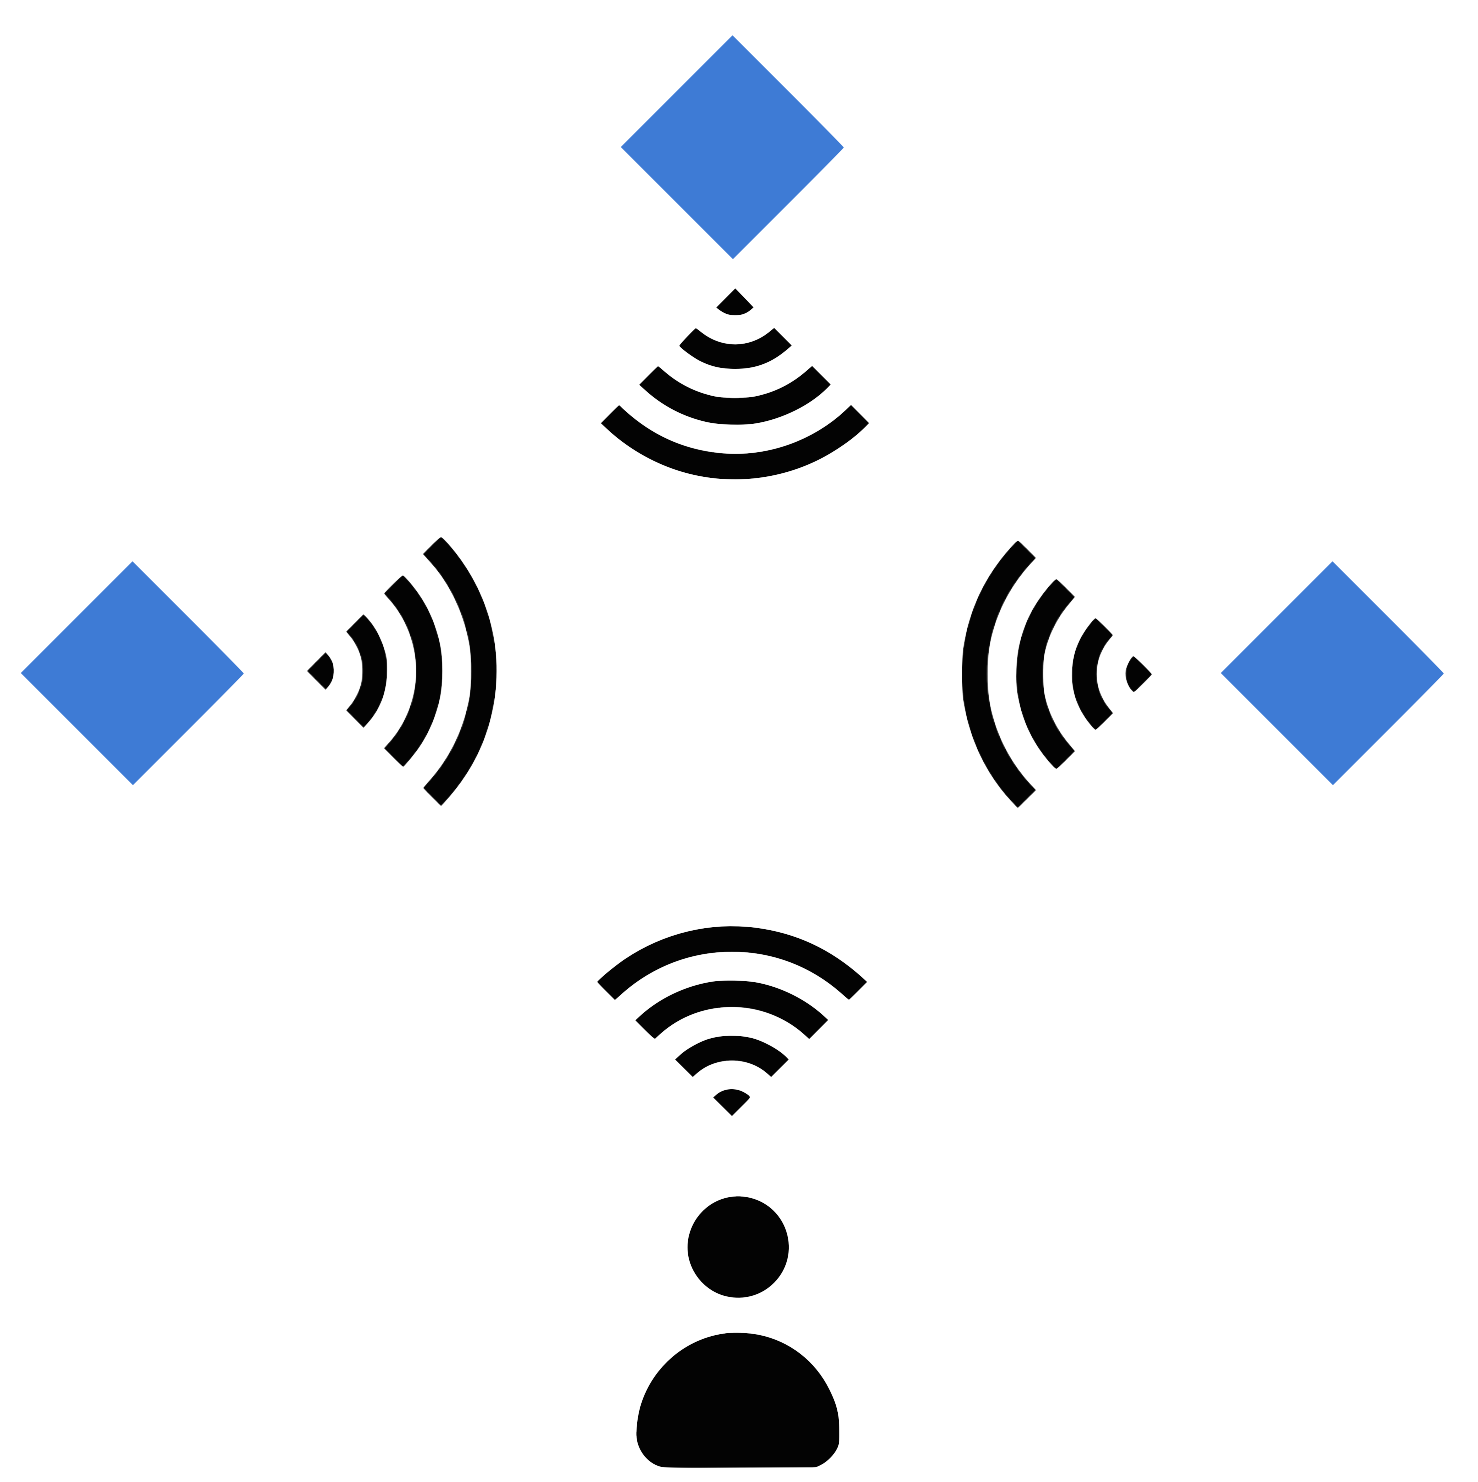
\includegraphics[width=0.5\textwidth]{images/new_model.png}
    \caption{Spark Driverless Model}\label{fig:new_model}
\end{figure}

% section background (end)
